\documentclass[crop,tikz,11pt]{standalone}
\usepackage[mathlf,mathtabular]{MinionPro}

\definecolor{seaborn_blue}{HTML}{4C72B0}

\begin{document}
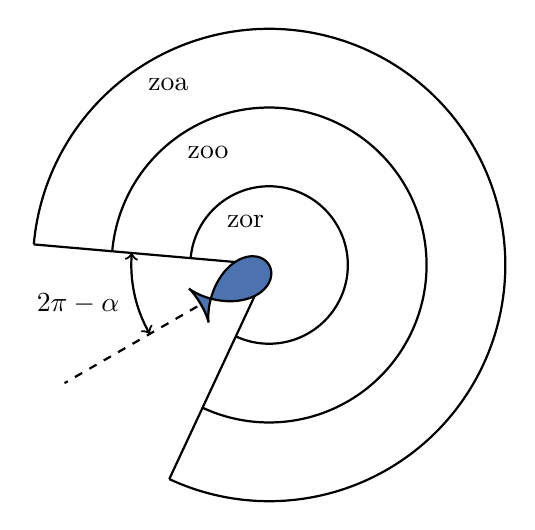
\begin{tikzpicture}[rotate=30]
	% draw zor
   \draw [thick, domain=0:145, samples=100] plot ({cos(\x)}, {sin(\x)});
   \draw [thick, domain=215:360, samples=100] plot ({cos(\x)}, {sin(\x)});
   % draw zoo
   \draw [thick, domain=0:145, samples=100] plot ({2*cos(\x)}, {2*sin(\x)});
   \draw [thick, domain=215:360, samples=100] plot ({2*cos(\x)}, {2*sin(\x)});
   %draw zoa
   \draw [thick, domain=0:145, samples=100] plot ({3*cos(\x)}, {3*sin(\x)});
   \draw [thick, domain=215:360, samples=100] plot ({3*cos(\x)}, {3*sin(\x)});
   % close circle segments
   \draw [thick] (0, 0) -- ({-3*sin(270-145)}, {-3*cos(270-145)});
   \draw [thick] (0, 0) -- ({3*sin(145-200)}, {-3*cos(145-200)});
   % line behind fish
   \draw [thick, dashed] (0, 0) -- (-3, 0);
   % make that sweet sweet fish curve
   \draw [fill=seaborn_blue, thick, domain=-200:200, samples=100] plot ({0.5*(cos(\x) - sin(\x)^2/1.41)-0.5}, {0.5*sin(\x)*cos(\x)});
   \node [text width=1cm] at (0.25, 0.5) {zor};
   \node [text width=1cm] at (0.25, 1.5) {zoo};
   \node [text width=1cm] at (0.25, 2.5) {zoa};
   % illustrate blind zone
   \draw [<->, thick, domain=145:180, samples=100] plot ({1.75*cos(\x)}, {1.75*sin(\x)});
   \node [text width=3cm] at (-1.5, 0.3) {$2\pi - \alpha$};
\end{tikzpicture}
\end{document}
